% This file was created with tikzplotlib v0.10.1.
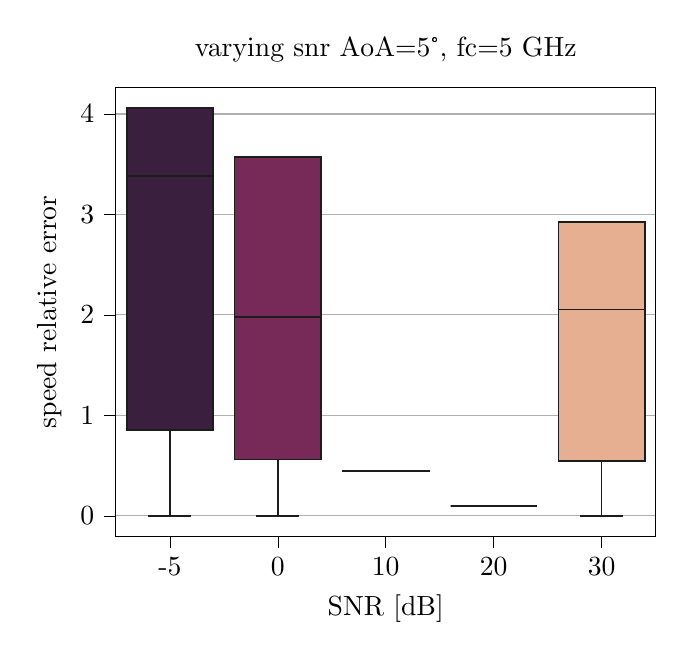
\begin{tikzpicture}

\definecolor{black28}{RGB}{28,28,28}
\definecolor{brown1814888}{RGB}{181,48,88}
\definecolor{burlywood231175145}{RGB}{231,175,145}
\definecolor{darkgray176}{RGB}{176,176,176}
\definecolor{darkslategray583162}{RGB}{58,31,62}
\definecolor{indianred21811088}{RGB}{218,110,88}
\definecolor{purple1194288}{RGB}{119,42,88}

\begin{axis}[
tick align=outside,
tick pos=left,
title={varying snr AoA=5°, fc=5 GHz},
x grid style={darkgray176},
xlabel={SNR [dB]},
xmin=-0.5, xmax=4.5,
xtick style={color=black},
xtick={0,1,2,3,4},
xticklabels={-5,0,10,20,30},
y grid style={darkgray176},
ylabel={speed relative error},
ymajorgrids,
ymin=-0.202824517828981, ymax=4.26000760898922,
ytick style={color=black}
]
\path [draw=black28, fill=darkslategray583162, semithick]
(axis cs:-0.4,0.853137966874885)
--(axis cs:0.4,0.853137966874885)
--(axis cs:0.4,4.05715160280555)
--(axis cs:-0.4,4.05715160280555)
--(axis cs:-0.4,0.853137966874885)
--cycle;
\path [draw=black28, fill=purple1194288, semithick]
(axis cs:0.6,0.560096175140716)
--(axis cs:1.4,0.560096175140716)
--(axis cs:1.4,3.57155182766178)
--(axis cs:0.6,3.57155182766178)
--(axis cs:0.6,0.560096175140716)
--cycle;
\path [draw=black28, fill=brown1814888, semithick]
(axis cs:1.6,0.445472965871995)
--(axis cs:2.4,0.445472965871995)
--(axis cs:2.4,0.445473104026297)
--(axis cs:1.6,0.445473104026297)
--(axis cs:1.6,0.445472965871995)
--cycle;
\path [draw=black28, fill=indianred21811088, semithick]
(axis cs:2.6,0.0973757660819709)
--(axis cs:3.4,0.0973757660819709)
--(axis cs:3.4,0.0973757661165538)
--(axis cs:2.6,0.0973757661165538)
--(axis cs:2.6,0.0973757660819709)
--cycle;
\path [draw=black28, fill=burlywood231175145, semithick]
(axis cs:3.6,0.544378456638495)
--(axis cs:4.4,0.544378456638495)
--(axis cs:4.4,2.92560086757766)
--(axis cs:3.6,2.92560086757766)
--(axis cs:3.6,0.544378456638495)
--cycle;
\addplot [semithick, black28]
table {%
0 0.853137966874885
0 0.000752000757596582
};
\addplot [semithick, black28]
table {%
0 4.05715160280555
0 4.05715160322475
};
\addplot [semithick, black28]
table {%
-0.2 0.000752000757596582
0.2 0.000752000757596582
};
\addplot [semithick, black28]
table {%
-0.2 4.05715160322475
0.2 4.05715160322475
};
\addplot [semithick, black28]
table {%
1 0.560096175140716
1 0.000225171057582635
};
\addplot [semithick, black28]
table {%
1 3.57155182766178
1 3.57155183190224
};
\addplot [semithick, black28]
table {%
0.8 0.000225171057582635
1.2 0.000225171057582635
};
\addplot [semithick, black28]
table {%
0.8 3.57155183190224
1.2 3.57155183190224
};
\addplot [semithick, black28]
table {%
2 0.445472965871995
2 0.445472759447081
};
\addplot [semithick, black28]
table {%
2 0.445473104026297
2 0.445473104026297
};
\addplot [semithick, black28]
table {%
1.8 0.445472759447081
2.2 0.445472759447081
};
\addplot [semithick, black28]
table {%
1.8 0.445473104026297
2.2 0.445473104026297
};
\addplot [semithick, black28]
table {%
3 0.0973757660819709
3 0.0973757660304337
};
\addplot [semithick, black28]
table {%
3 0.0973757661165538
3 0.0973757661165538
};
\addplot [semithick, black28]
table {%
2.8 0.0973757660304337
3.2 0.0973757660304337
};
\addplot [semithick, black28]
table {%
2.8 0.0973757661165538
3.2 0.0973757661165538
};
\addplot [semithick, black28]
table {%
4 0.544378456638495
4 3.14879354829399e-05
};
\addplot [semithick, black28]
table {%
4 2.92560086757766
4 2.92560086832979
};
\addplot [semithick, black28]
table {%
3.8 3.14879354829399e-05
4.2 3.14879354829399e-05
};
\addplot [semithick, black28]
table {%
3.8 2.92560086832979
4.2 2.92560086832979
};
\addplot [semithick, black28]
table {%
-0.4 3.38235292514963
0.4 3.38235292514963
};
\addplot [semithick, black28]
table {%
0.6 1.9759800681607
1.4 1.9759800681607
};
\addplot [semithick, black28]
table {%
1.6 0.445473104024746
2.4 0.445473104024746
};
\addplot [semithick, black28]
table {%
2.6 0.0973757661165532
3.4 0.0973757661165532
};
\addplot [semithick, black28]
table {%
3.6 2.05485609172377
4.4 2.05485609172377
};
\end{axis}

\end{tikzpicture}
